\section{Zielpunktgewinnung \dcsecondauthorshort}
Um den Zielpunkt für den implementierten \glqq Pure-Pursuit\grqq -Regler zu erhalten, müssen die nachfolgend beschriebenen Schritte ausgeführt werden.

\subsection{Holen der benötigten Punkte aus der Weltkarte}
Im gewählten Fahrspurverfolgungskonzept läuft die Erkennung der Fahrbahnmarkierungen und die Regelung des Fahrzeugs asynchron ab, beide Komponenten kommunizieren nur über eine Weltkarte miteinander. Somit muss vor jedem Regelzyklus festgestellt werden, welche Punkte dieser Weltkarte zum Steuern des Roboters noch relevant sind. Hierfür wurden einige Regeln festgelegt:
\begin{enumerate}
\item
Der Zeitpunkt, an welchem die Punkte in die Weltkarte eingetragen wurden, muss aktuell genug sein.
\item \label{item:regelung:zielpunkt:holen:regeln:abstand}
Der Abstand (analog \ref{eq:norm:distpoints}) der aktuellen Roboterpose zur Pose, an welcher die Punkte in die globale Karte eingetragen wurden, darf einen Grenzwert nicht überschreiten.
\item \label{item:regelung:zielpunkt:holen:regeln:xcoord}
Die x-Koordinate der in das Roboter-\gls{acr:ks} \gls{lat:RoboterKOS} transformierten Punkte muss in einem bestimmten Intervall liegen.
\end{enumerate}
Um die Punkte nach Kategorie \ref{item:regelung:zielpunkt:holen:regeln:xcoord} filtern zu können und später zur Regelung zu nutzen, werden sie nach Schritt \ref{item:regelung:zielpunkt:holen:regeln:abstand} vom Welt-\gls{acr:ks} \gls{lat:WeltKOS} in Roboterkoordinaten (\gls{acr:ks} \gls{lat:RoboterKOS}) transformiert.

\subsection{Kreissegment-Fit} \label{regelung:zielpunkt:kreissegment-fit}
Um später alle drei Fahrbahnmarkierungen zur Zielpunktgewinnung in die gewünschte Fahrspur verschieben zu können, muss eine mathematische Repräsentation der Mittellinie und Seitenlinien gefunden werden, welche dies erlaubt. Da in der Weltkarte aus mehreren Bildern erkannte Punkte vorhanden sind, soll ein zu allen diesen Frames möglichst gut passender Zielpunkt gefunden werden. Wählt man den Bereich der für die Zielpunktfindung relevanten Fahrbahnmarkierungen nicht zu groß, kann deren Verlauf gut durch Kreisbögen approximiert werden. 

\subsubsection{Kreisfit} 
Zur Ermittlung des optimalen Kreises durch die gefragten Punkte wurde der Taubin-Kreisfit \autocite{taubinEstimationPlanarCurves1991} in der Implementierung von \autocite{nikolaichernovMATLABCodesFitting} verwendet. 

\subsubsection{Ermittlung zusätzlicher Parameter}
Neben dem Mittelpunkt \gls{lat:mp} und Radius \gls{lat:rad} muss zur vollständigen Parameterisierung des Kreisbogens Start- und Endwinkel sowie die Drehrichtung des Bogens bekannt sein.

\paragraph{Start- und Endwinkel}
Zur Ermittlung des Startwinkels \( \varphi_s \) wird vom Mittelpunkt des Kreises \gls{lat:mp} zum Punkt \pnt{p_s} ein Vektor \vct{o_s} aufgespannt. \pnt{p_s} stellt den Punkt mit dem geringsten Abstand vom Koordinatenursprung des Roboter-\gls{acr:ks} \gls{lat:RoboterKOS} aus der Koordinatenserie, welche zum Kreisfit genutzt wurde, dar. Der gesuchte Startwinkel ergibt sich als:
\begin{equation}
\varphi_s =
\atantwo{\scl{o_{sy}, o_{sx}}} = 
\atantwo{\scl{p_{sy}-m_{y}, p_{sx}-m_{x}}}
\end{equation}
Zur Ermittlung des Endwinkels \( \varphi_e \) wird analog unter Nutzung des Punktes mit dem größten Abstand vom Koordinatenursprung des Roboter-\gls{acr:ks} \gls{lat:RoboterKOS} verfahren.

\begin{figure}[htb]
  \centering
  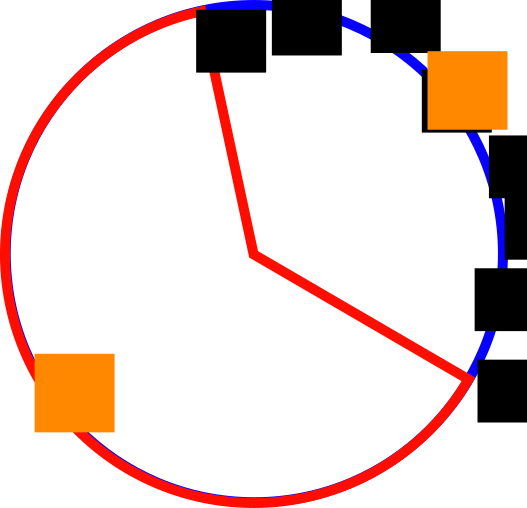
\includegraphics[width=0.75\textwidth]{regelung_zielpunkt_betweenpoint}
  \caption{Ermittlung der Rotationsrichtung}
  \label{fig:regelung:zielpunkt:betweenpoint}
\end{figure}

\paragraph{Rotationsrichtung}
Die Methode zur Ermittlung der Rotationsrichtung orientiert sich an \autocite{drauschkeEchtzeitfaehigeStartpunktalgorithmenFuer2016}. Es wird der Punkt \pnt{p_{b1}} \eqref{eq:regelung:betweenpoint} auf dem Radius des Kreises mit dem Winkel \(  \varphi_{b1} = (\varphi_s + \varphi_e)/2 \) errechnet.
Desweiteren wird der Punkt \pnt{p_{b2}} \eqref{eq:regelung:betweenpoint}auf dem Radius des Kreises mit dem Winkel \(  \varphi_{b2} = (\varphi_s + \varphi_e)/2 + \pi \) bestimmt.
\begin{equation} \label{eq:regelung:betweenpoint}
\pnt{p_{b1/2}} = \pnt{m} + 
\begin{pmatrix}
\cos{\varphi_{b1/2}} \\
\sin{\varphi_{b1/2}}
\end{pmatrix}
\cdot \gls{lat:rad}
\end{equation}
Aus den Mittelwerten \( \mean{\nrm{\gls{lat:av}}}_{1/2} \) \eqref{eq:regelung:betweenpointmeandistances} der Abstände \( \nrm{\gls{lat:av}}_{1/2i} = \nrm{\pnt{p_{b1/2}} - \pnt{p_{\text{fit}i}}} \) (analog \ref{eq:norm:distpoints}) der \(n\) zum Kreisfit genutzten Punkte \(\pnt{p_{\text{fit}i}}\) zu den Punkten \(\pnt{p_{b1}}\) und \(\pnt{p_{b2}}\) kann nun die Rotationsrichtung bestimmt werden.
\begin{equation} \label{eq:regelung:betweenpointmeandistances}
\mean{\nrm{\gls{lat:av}}}_{1/2} = \frac{\sum_{i=1}^n \nrm{\gls{lat:av}}_{1/2i}}{n} 
\end{equation}
\begin{tabular}{ccc}
& \(\mean{\nrm{\gls{lat:av}}}_{1}<\mean{\nrm{\gls{lat:av}}}_{2}\) & 
\(\mean{\nrm{\gls{lat:av}}}_{1}\geq \mean{\nrm{\gls{lat:av}}}_{2}\) \\
\(\varphi_s<\varphi_e\) &  mathematisch positiver Drehsinn & mathematisch negativer Drehsinn \\
\(\varphi_s\geq \varphi_e\) &  mathematisch negativer Drehsinn & mathematisch positiver Drehsinn
\end{tabular}

\begin{figure}[htb]
  \centering
  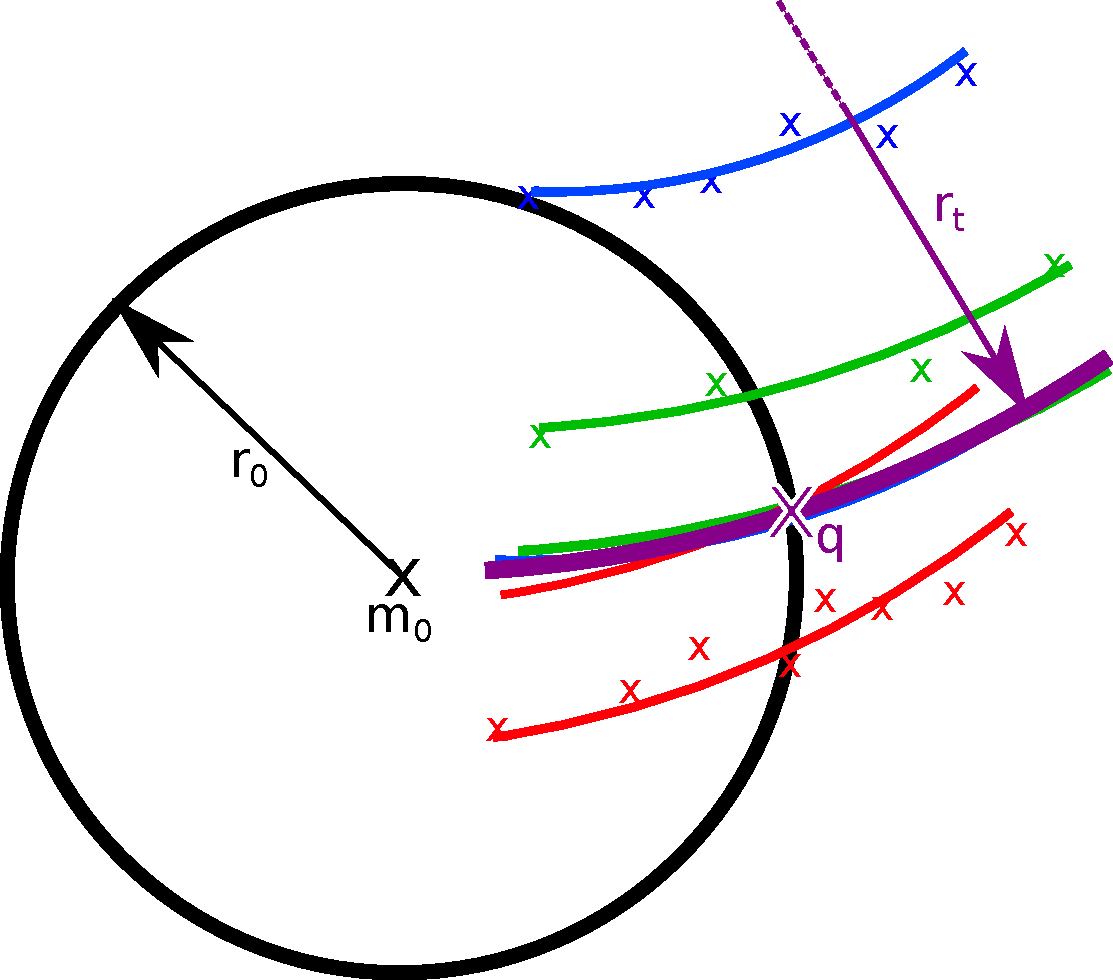
\includegraphics[width=0.75\textwidth]{regelung_zielpunkt_prinzip}
  \caption{Zielpunktgewinnung}
  \label{fig:regelung:zielpunkt:zielpunktgewinnung}
\end{figure}

\subsection{Verschiebung der Kreissegmente}
Um die drei gefundenen Kreissegmente zur Gewinnung eines Zielpunktes nutzen zu können, müssen diese um die halbe bzw. anderthalbe Fahrspurbreite verschoben werden. Hierfür muss je nach Rotationsrichtung des Kreissegments und gewünschter Fahrbahn (links/rechts) der Radius des Kreissegments modifiziert werden. Zur genauen Aufschlüsselung dieser Logik sei der Leser auf den Quellcode verwiesen. REFERENZ

\subsection{Bildung des Trajektorienkreissegments}
Um aus den drei in die Fahrspur verschobenen Segmenten einen Kreisbogen zu erhalten, werden die in die Fahrspur verschobenen Kreissegmente nun gesampelt. Von jedem Kreissegment werden so viele Punkte abgetastet, wie zur Berechnung seiner Parameter genutzt wurden. Die so entstandene Koordinatenserie bildet die Basis für den Fit des Trajektoriekreisbogens. Hierfür wird dieselbe Prozedur wie in  \ref{regelung:zielpunkt:kreissegment-fit} verwendet.

\subsection{Schnittpunktberechnung}
Um eine möglichst gleichmäßige Regelung des Lenkwinkels zu ermöglichen, sollte der Zielpunkt \gls{lat:zp}  der \glqq Pure-Pursuit\grqq -Regelung in jeder Fahrsituation den gleichen Abstand vom Ursprung des Roboter-\gls{acr:ks} \gls{lat:RoboterKOS} besitzen (die sogenannte Lookahead-Distance). \gls{lat:zp} muss sich also auf dem Kreis mit Mittelpunkt \(\pnt{\gls{lat:mp}_0}=(0,0)\) und Radius \(\gls{lat:rad}_0\) gleich der Lookahead-Distance befinden. Da \gls{lat:zp} ebenfalls  auf dem Trajektorienkreissegment mit Mittelpunkt \(\pnt{\gls{lat:mp}_t}\) und Radius \( \gls{lat:rad}_t\) liegt, reduziert sich die Zielpunktermittlung auf die Schnittpunktberechnung zweier Kreise \autocite{Schnittpunkt2018}:
\begin{subequations}
\begin{equation}
\pnt{\gls{lat:zp}_{1/2}}=\pnt{\gls{lat:mp}_0} + \vct{d_1} \pm l \cdot \vct{e_2}
\end{equation}
\begin{equation}
\vct{e_2} = \begin{pmatrix} -\scl{e_{1y}} \\ \scl{e_{1x}} \end{pmatrix}
\end{equation}
\begin{equation}
\vct{e_1} = \begin{pmatrix} \scl{e_{1x}} \\ \scl{e_{1y}} \end{pmatrix} =
\frac{\pnt{\gls{lat:mp}_t}-\pnt{\gls{lat:mp}_0}}{\nrm{ \pnt{\gls{lat:mp}_t}-\pnt{\gls{lat:mp}_0}}}
\end{equation}
\begin{equation}
\vct{d_1} = \begin{pmatrix} \scl{d_{1x}} \\ \scl{d_{1y}} \end{pmatrix} =
\frac{1}{2} \cdot \left( \frac{\gls{lat:rad}_t-\gls{lat:rad}_0}{\nrm{\pnt{\gls{lat:mp}_t}-\pnt{\gls{lat:mp}_0}}^2}+1 \right)
\cdot (\pnt{\gls{lat:mp}_t}-\pnt{\gls{lat:mp}_t})
\end{equation}
\begin{equation}
l = \sqrt[2]{\gls{lat:rad}_0^2-\nrm{\vct{d_0}}^2} = \sqrt[2]{\gls{lat:rad}_t^2-\nrm{\vct{d_t}}^2}
\end{equation}
\end{subequations}
Da zwei sich schneidende Kreise zwei Schnittpunkte besitzen, muss nun geprüft werden,  welcher der Schnittpunkte auf dem gültigen Segment des Trajektorienkreises liegt. Dies kann anhand von Start- und Endwinkel sowie dessen Rotationsrichtung ermittelt werden und ist im Quelltext REFERENZ genauer nachzulesen.

